% !TEX program = pdflatex
% !TEX options = -synctex=1 -interaction=nonstopmode -file-line-error "%DOC%"
% Computational Physics Assignment 2
\documentclass[UTF8,10pt,a4paper]{article}
\usepackage{ctex}
\newcommand{\CourseName}{Computational Physics}
\newcommand{\CourseCode}{PHYS1504}
\newcommand{\Semester}{Spring, 2020}
\newcommand{\ProjectCode}{Assignment 2}
\newcommand{\ProjectName}{Density-Functional Calculation of Stanene}
\newcommand{\DueTimeType}{Due Time}
\newcommand{\DueTime}{12:00, April 27, 2020 (Sunday)}
\newcommand{\StudentName}{陈稼霖}
\newcommand{\StudentID}{45875852}
\usepackage[vmargin=1in,hmargin=.5in]{geometry}
\usepackage{fancyhdr}
\usepackage{lastpage}
\usepackage{calc}
\pagestyle{fancy}
\fancyhf{}
\fancyhead[L]{\CourseName}
\fancyhead[C]{\ProjectCode}
\fancyhead[R]{\StudentName}
\fancyfoot[R]{\thepage\ / \pageref{LastPage}}
\setlength\headheight{12pt}
\fancypagestyle{FirstPageStyle}{
    \fancyhf{}
    \fancyhead[L]{\CourseName\\
        \CourseCode\\
        \Semester}
    \fancyhead[C]{{\large\bfseries\ProjectCode}\\
        {\large\bfseries\ProjectName}\\
        \DueTimeType\ : \DueTime}
    \fancyhead[R]{Name : \makebox[\widthof{\StudentID}][s]{\StudentName}\\
        Student ID\@ : \StudentID\\
        Score : \underline{\makebox[\widthof{\StudentID}]{}}}
    \fancyfoot[R]{\thepage\ / \pageref{LastPage}}
    \setlength\headheight{36pt}
}
\usepackage{amsmath,amssymb,amsthm,bm}
\allowdisplaybreaks[4]
\newtheoremstyle{Problem}
{}
{}
{}
{}
{\bfseries}
{.}
{ }
{\thmname{#1}\thmnumber{ #2}\thmnote{ (#3)} Score: \underline{\qquad\qquad}}
\theoremstyle{Problem}
\newtheorem{prob}{Problem}
\newtheoremstyle{Solution}
{}
{}
{}
{}
{\bfseries}
{:}
{ }
{\thmname{#1}}
\makeatletter
\def\@endtheorem{\qed\endtrivlist\@endpefalse}
\makeatother
\theoremstyle{Solution}
\newtheorem*{sol}{Solution}
\providecommand{\abs}[1]{\left\lvert#1\right\rvert}
\usepackage{graphicx}
\usepackage{subfigure}
\begin{document}
\thispagestyle{FirstPageStyle}
\begin{prob}[Density-Functional Calculation of Stanene (total points: 20)]
    In the past fifteen years, the discovery of topological insulators has revolutionized the conventional viewpoint of the stats of matter. In addition to metal, semiconductor and insulator classified in solid-physics by their unique electronic structure, topological insulators demonstrate a completely different picture, whose bulk behave like a normal semiconductor/insulator with well defined gap. However, on their surface/edges there exists nondissipative charge/spin current, making the topological insulator a new state of matter that cannot be understood by conventional band theory.

    It now becomes clear that the unique nature of the topological insulators is deeply related to their nontrivial berry curvature which, for a long time, has been believed to be unimportant. There exists many materials demonstrating certain level of topological properties. In this exercise, you will examine one simple yet very interesting topological insulator. \textit{i.e.} stanene - a monolayer Sn atoms with honeycomb structure.

    Please carefully read "Large-Gap Quantum Spin Hall insulators in Thin Films" by Yong Xu et al, at Phys. Rev. Lett. \textbf{111}, 136804 (2013) and try to repeat figure 2 and figure 4. To be more specific, you are about to do
    \begin{enumerate}
        \item[1.] Construct the crystal model for stanene. You can refer to figure 1c for the lattice constants and relaex the internal coordinates of Sn atoms automatically with DFT. Similar to the first example discussed during the lecture (\verb|https://cms.mpi.univie.ac.at/wiki/index.php/Fcc_Si|), to get the lattice constant precisely, you need to try different values of the lattice constant and look for the one with the lowest energy.
        \item[2.] Calculate the bulk electronic structure for the three cases shown in figure 2(a-c). Note that, for each case, one need to first generate the corresponding relaxed structure based on which the electronic structure is calculated.
        \item[3.] Constant slab geometry for stanene, fluorinated statnene and stanane, and calculate their edge states as shown in figure 4 (a-c).
    \end{enumerate}
    \textbf{Note that, the slab calculations (figure 3) takes long time to finish, please start your job as early as possible.}
\end{prob}
\begin{sol}
    \begin{enumerate}
        \item[1.] \textbf{计算步骤}(所有的配置文件见压缩包附件):
        \begin{enumerate}
            \item 参考文献图1(c),stanene的晶格常数大约在[$4.65$\AA,$4.7$\AA]范围内,因此将晶格常数$a$遍历($4.64$\AA,$4.65$\AA,$4.66$\AA,\\$4.67$\AA,$4.68$\AA,$4.69$\AA,$4.70$\AA,$4.71$\AA,$4.72$\AA)这$11$个值,同时将一个原胞内两个Sn原子在$c$方向的高度差$z$遍历($0.00$\AA,\\$0.10$\AA,$0.16$\AA,$0.17$\AA,$0.18$\AA,$0.19$\AA,$0.20$\AA)这7个值,分别计算体系的能量,结果如图\ref{1-1-1},因此stanene的稳定结构的晶格常数在$0.66$\AA左右,原胞中两个Sn原子的高度差在$0.19$\AA左右;
            \item 进一步查找stanene的稳定结构:将晶格常数$a$遍历($4.652$\AA,$4.654$\AA,$4.656$\AA,$4.658$\AA)这$4$个值,同时将在一个原胞内两个Sn原子在$c$方向的高度差$z$遍历($0.184$\AA,$0.188$,$0.192$\AA,$0.196$\AA)这四个数,分别计算体系的能量,结果如图\ref{1-1-2}.
        \end{enumerate}
        \begin{figure}[h]
            \centering
            \subfigure[]{
            \label{1-1-1}
            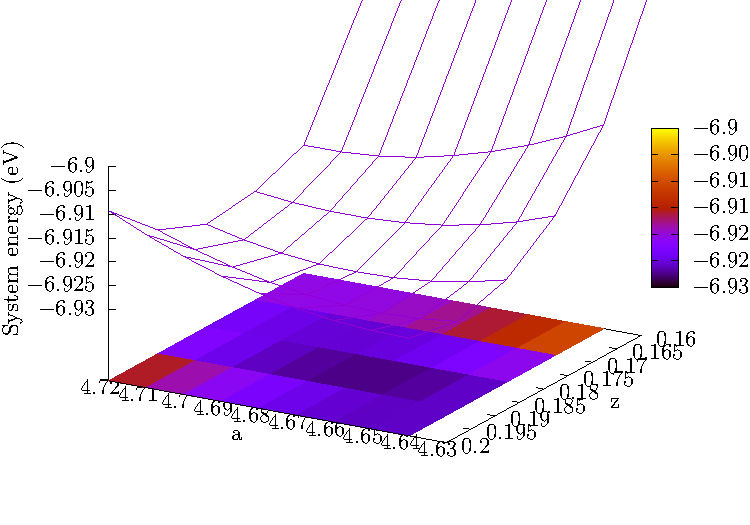
\includegraphics[width=.45\textwidth]{1-1-1.pdf}}
            \subfigure[]{
            \label{1-1-2}
            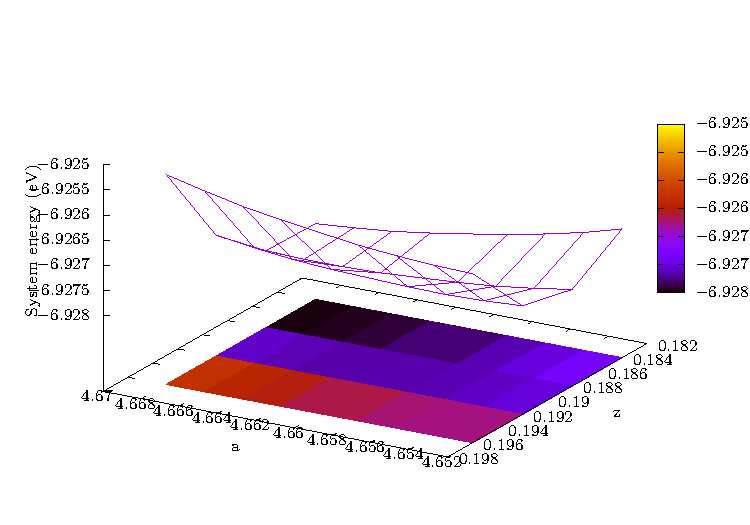
\includegraphics[width=.45\textwidth]{1-1-2.pdf}}
        \end{figure}
        \textbf{计算结果}:stanene的稳定结构的晶格常数为$4.666$\AA,原胞中两个Sn原子的高度差为$0.196$\AA.
        \item[2.] \textbf{计算步骤}:\\
        对于stanene,尝试直接用前一题得到的晶体结构计算能带结构,发现计算得到的能带结构的带隙不在费米面上(图略),推测应该是因为晶体结构不够准确造成了较大的误差,因此:
        \begin{enumerate}
            \item 在第一题计算的结果基础上,设置ISIF$=3$(同时调整原胞内原子位置,原胞形状和原胞大小),NSW$=20$(迭代循环$20$次)进一步计算晶体的稳定结构;
            \item 将上一步得到的晶体结构(储存在CONTCAR中)写入POSCAR中,进行自洽计算;
            \item 用自洽计算得到的电子密度(存储在CHGCAR中)计算能带结构.
        \end{enumerate}
        对于fluorinated stanene和stanane,由于ISIF=3会直接调整原胞形状,在这两种晶体的结构还不能大致确定的情况下,可能会较为剧烈地破坏晶体的对称性,因此不应该直接设置ISIF=3进行计算,而应该:
        \begin{enumerate}
            \item 先根据论文中提供的数据假定晶体结构(对fluorinated stanene,假定晶格常数为$5.025$\AA,对stanane,假定晶格常数为$4.72$\AA,对两种情况,均设修饰原子位于最近的Sn原子正上/下方$0.2$\AA处),设置ISIF$=2$(仅会调整原胞内原子的位置),NSW$=10$计算晶体的稳定结构;
            \item 将上一步得到的晶体结构写入POSCAR中,设置ISIF$=3$,NSW$=10$进一步计算晶体的稳定结构;
            \item 将上一步得到的晶体结构写入POSCAR中,进行自洽计算;
            \item 用自洽计算得到的电子密度计算能带结构.
        \end{enumerate}
        \textbf{计算结果}:三种材料的稳定结构的参数如表\ref{1-2-T}.
        \begin{table}[h]
            \centering
            \caption{三种材料的稳定结构的参数}
            \label{1-2-T}
            \begin{tabular}{c|ccccll}
            材料名称 & \multicolumn{2}{c}{stanene} & \multicolumn{2}{c}{fluorinated stanene} & \multicolumn{2}{c}{stanane} \\ \hline
            是否自旋轨道耦合 & 是 & 否 & 是 & 否 & \multicolumn{1}{c}{是} & \multicolumn{1}{c}{否} \\
            晶格常数/\AA & $4.66636$ & $4.68645$ & $5.00161$ & $5.02374$ & $4.73828$ & $4.71886$ \\
            \begin{tabular}[c]{@{}c@{}}修饰原子与最近的Sn原子\\ 的平均距离/\AA\end{tabular} & - & - & $1.97533$ & $1.96765$ & $1.73530$ & $1.73944$
            \end{tabular}
            \end{table}

        三种材料的体能带结构如图\ref{1-2-F}.
        \begin{figure}[h]
            \centering
            \subfigure[]{
            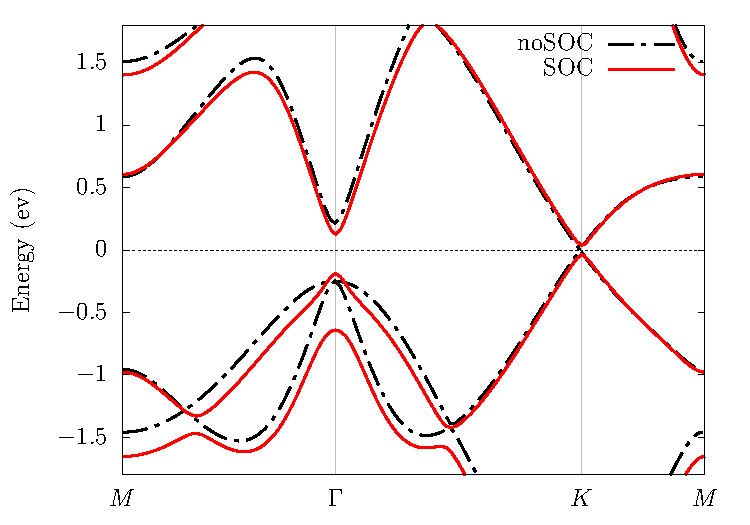
\includegraphics[width=.32\textwidth]{1-2-stanene.pdf}}
            \subfigure[]{
            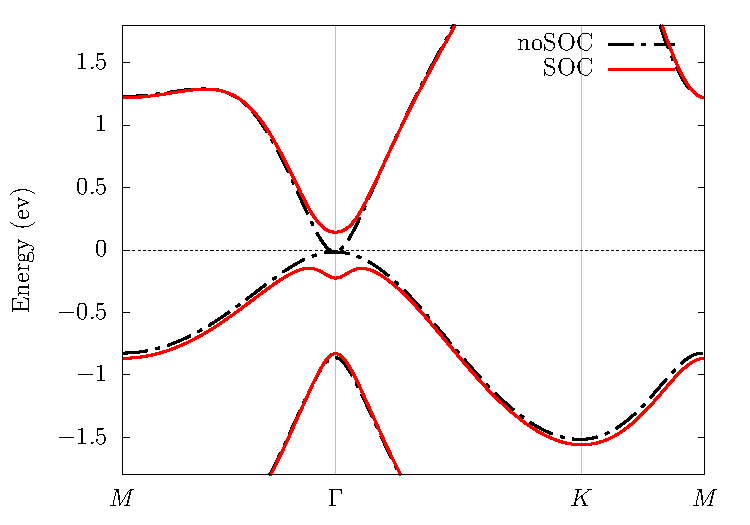
\includegraphics[width=.32\textwidth]{1-2-stanene-F.pdf}}
            \subfigure[]{
            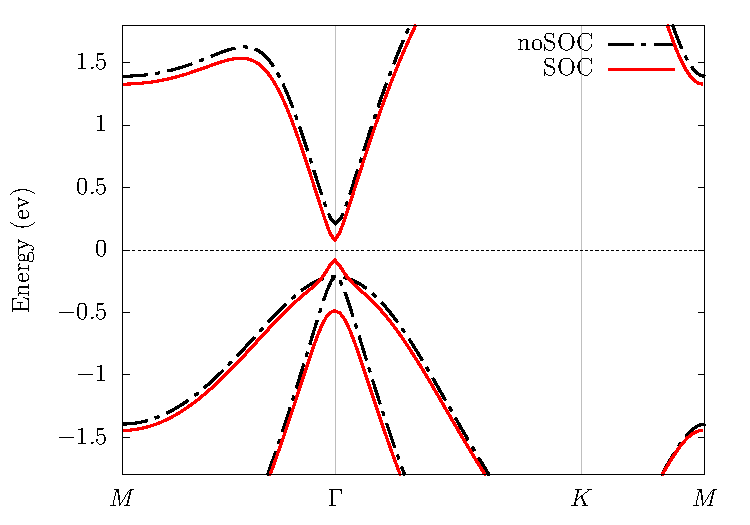
\includegraphics[width=.32\textwidth]{1-2-stanane.pdf}}
            \caption{无旋轨道耦合(黑色点划线)和有自旋轨道耦合(红色实线)的 (a) stanene, (b) fluorinated stanene, (c) stanane 的能带结构.}
            \label{1-2-F}
        \end{figure}

        \textbf{讨论}:根据计算结果,加上修饰原子会增加Sn-Sn键的键长,且使二维Sn平面的buckling减小,这或许说明了每个Sn的最近的修饰原子对与该Sn原子相邻的其他Sn原子有排斥作用.\\
        根据计算结果,不考虑自旋轨道耦合,stanene在$K$点具有交叉的能带,当考虑自旋轨道耦合,$K$的交叉能带被打开,且加上修饰原子后,带隙会显著增大.
        \item[3.] \textbf{计算步骤}:
        \begin{enumerate}
            \item 在上一题得到的三种材料的晶体结构的基础上,将$a$方向上的宽度拓展成原来$10$倍;
            \item 对拓展而成的nanoribbon做自洽计算,为了节省内存和时间,下调了ENCUT和kpoints的数量,上调了EDIFF;
            \item 用自洽计算得到的电子密度计算从$\Gamma$点$(0,0,0)$到$X'$点$(0,0.1,0)$的能带结构.
        \end{enumerate}
        \textbf{计算结果}:三种材料的slab的能带结构如图\ref{1-3-F}.
        \begin{figure}[h]
            \centering
            \subfigure[]{
            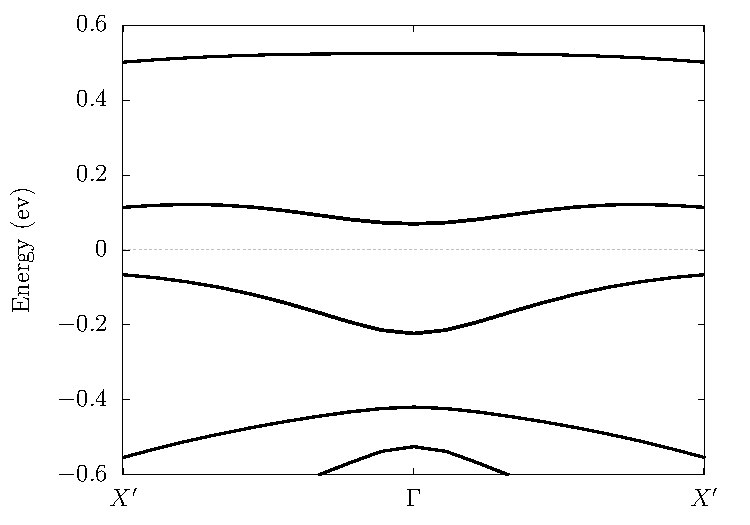
\includegraphics[width=.32\textwidth]{1-3-stanene.pdf}}
            \subfigure[]{
            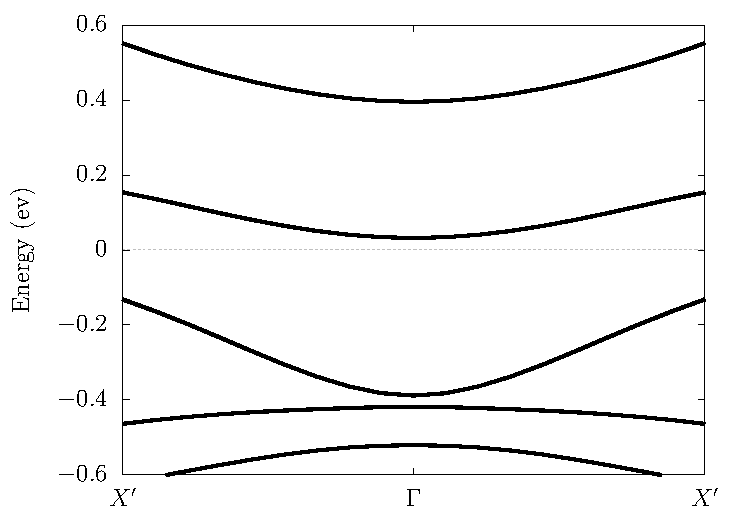
\includegraphics[width=.32\textwidth]{1-3-stanene-F.pdf}}
            \subfigure[]{
            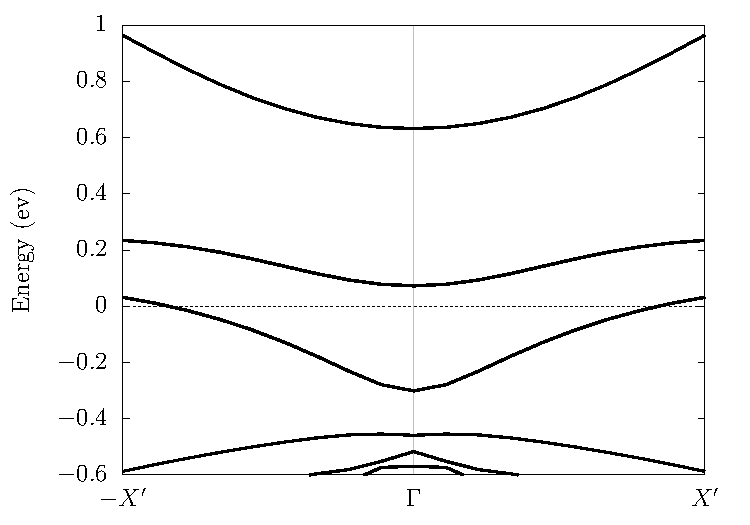
\includegraphics[width=.32\textwidth]{1-3-stanane.pdf}}
            \caption{(a) stanene, (b) fluorinated stanene, (c) stanane 的slab的能带结构.}
            \label{1-3-F}
        \end{figure}

        \textbf{讨论}:可能是由于计算精度不够,计算结果与论文有偏差,三种材料的slab均没有相交的能带,存在带隙,fluorinated stanene带隙很小,或许精度足够的情况下可以计算出相交的能带. \\
        计算得到能带比论文中疏很多,可能是因为取的slab的宽度比论文中小.\\
        这些slab的带隙并没有在费米面上(尽管用的是自洽计算得到的费米面),这可能是由于计算时ENCUT设得较低,kpoint取的较少导致的误差.\\
    \end{enumerate}
\end{sol}
\end{document}